\section{Latent Semantic Analysis (LSA) Experiment}\label{Latent Semantic Analysis Experiment (LSA) Experiment}

We stellen nu een proefopstelling op en we gaan het de vector space methode bij text mining toepassen op een echt voorbeeld.

\subsection{Proefopstelling}\label{Proefopstelling}
Als eerste verkrijgen we onze trainingsset door de polarity v2 dataset (website: http://www.cs.cornell.edu/People/pabo/movie-review-data) te downloaden. Deze dataset bevat positieve en negatieve reviews van imdb. We hebben te maken met supervised learning, want we weten welke reviews positief en welke negatief zijn. Het doel van het experiment is door middel van de geziene technieken zoals de vector space methode met latent semantic analysis en term weighting een inzicht te krijgen in de dataset en we proberen gelijkaardige reviews te groeperen. Tenslotte onderzoeken we de hypothese, waarbij we zeggen hoe meer features we hebben voor een document, hoe groter de nauwkeurigheid bij de classificatie.


\subsection{Werkwijze}\label{Werkwijze}

De werkwijze verloopt als volgt.

Eerst passen we document pre-processing toe. We halen alle stopwoorden en leestekens uit te dataset. Vervolgens stellen we een document-term matrix op. Dan optimaliseren we deze matrix voor classficatie door de matrix om te vormen naar een tf-idf matrix. Dit is de techniek waarbij we iedere frequentie $f_{ij}$ van een woord $w_{i}$ vervangen door de tf-idf score van het woord. Daaropvolgend reduceren we dimensie van onze tf-idf matrix naar 2 de latent semantic methode toe te passen. Iedere review wordt na de reductie voorgesteld door middel van 2 features. 
De reviews plotten we dan met elke review als een punt met een andere kleur voor positieve en negatieve reviews.
Ten slotte nemen we terug onze tf-idf matrix en reduceren het naar door een bepaald aantal features bijvoorbeeld 10, 50, 100, 500. En we kijken of onze hypothese geld waarbij we betere classificatie resultaten krijgen bij meer features.

\subsection{Resultaten}\label{Resultaten}

Als resultaat zien we dat het invoeren van term weighting zoals de tf-idf matrix echt wel nut heeft voor dat we de latent semantic methode toepassen.
Als we de 2 plots vergelijken, de ene zonder term weighting dan andere met term weighting, zien we duidelijk dat we bij diegene met term weighting duidelijk twee groepen kunnen onderscheiden.

\begin{figure}%
    \centering
    \subfloat[label 1]{{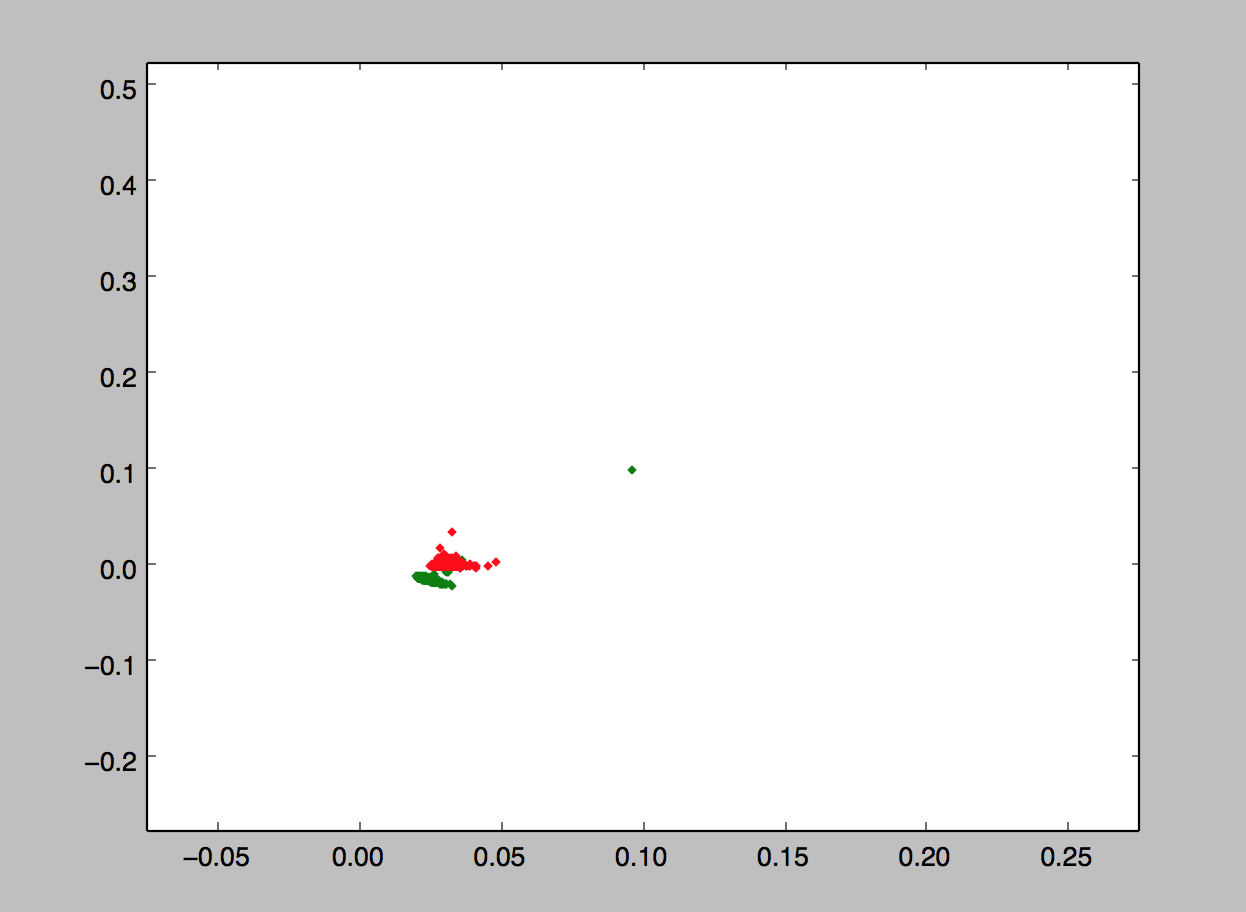
\includegraphics[width=5cm]{experiment_1} }}%
    \qquad
    \subfloat[label 2]{{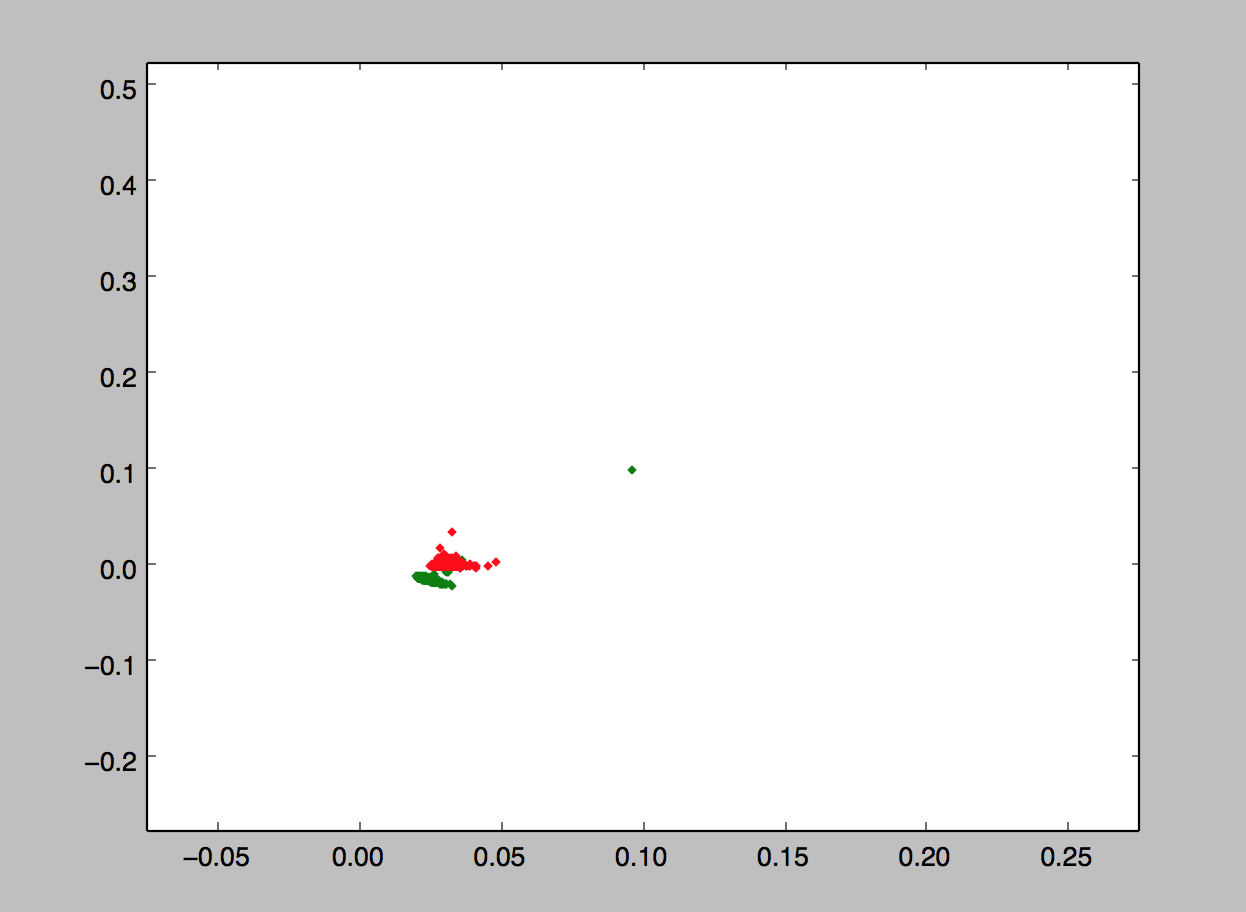
\includegraphics[width=5cm]{experiment_1} }}%
    \caption{2 Figures side by side}%
    \label{fig:example}%
\end{figure}

Tenslotte kunnen we ook onze hypthese bevestigen. We zien dat de hoeveelheid aan features, de nauwkeurigheid van de classificatie beïnvloed. Onderstaande afbeelding geeft deze relatie weer. De x-waarde stelt het aantal gelijkaardige reviews dat men opvraagt voor. De y-waarde geeft aan hoeveel er gemiddeld effectief juist geclassifiseerd zijn. Belangrijk om te weten is dat de dataset voor de helft uit positieve reviews bestaat en voor de helft uit negatieve. We trachten dus bij de classificatie een gemiddeld percentage van 50 percent te halen en we zien dat op onderstaand voorbeeld de lijn van 500 features hier het beste in slaagt.


\begin{center}
  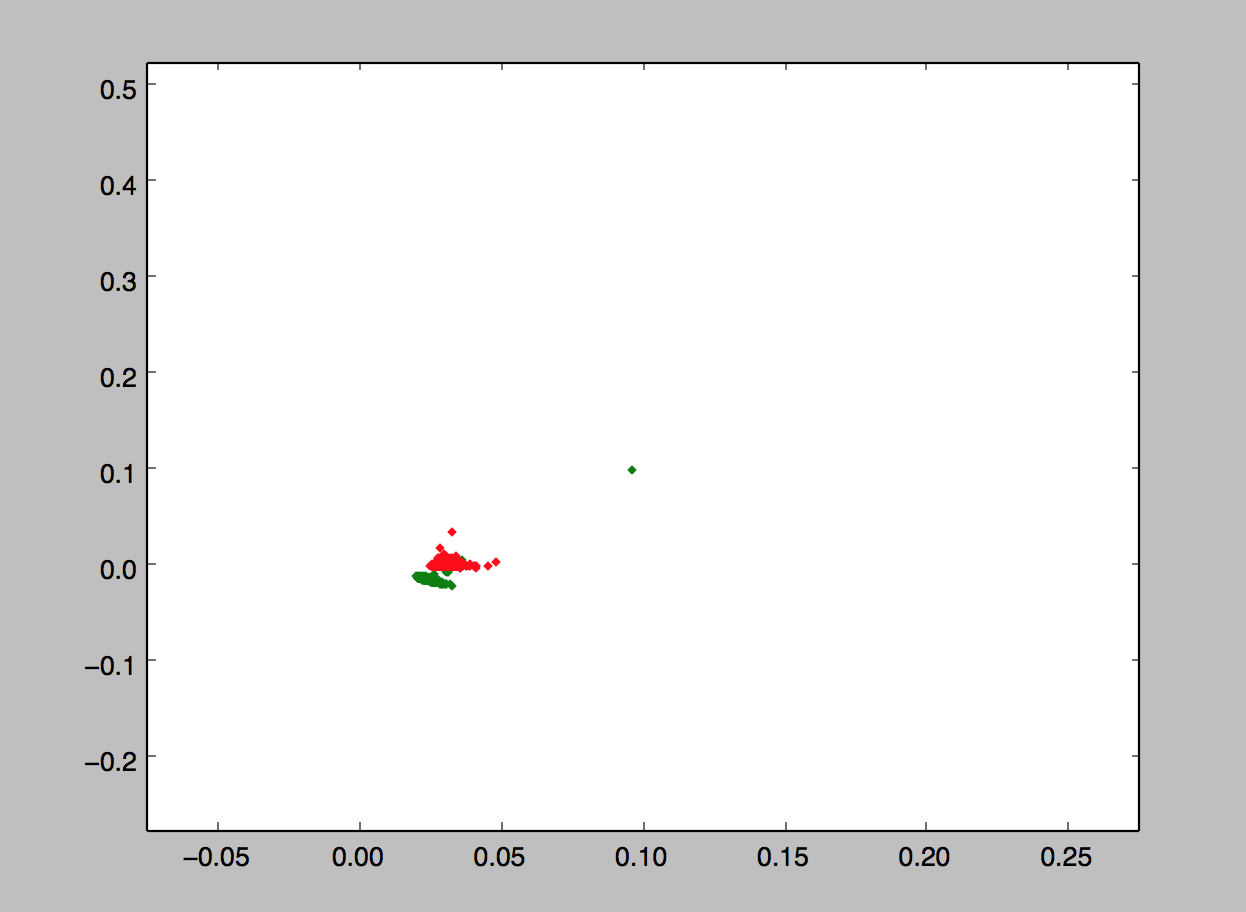
\includegraphics[width=10cm]{experiment_1}
  \captionof{figure}{Driedimensionale weergave van de kostfunctie}
\end{center}